\begin{figure*}
    \centering
    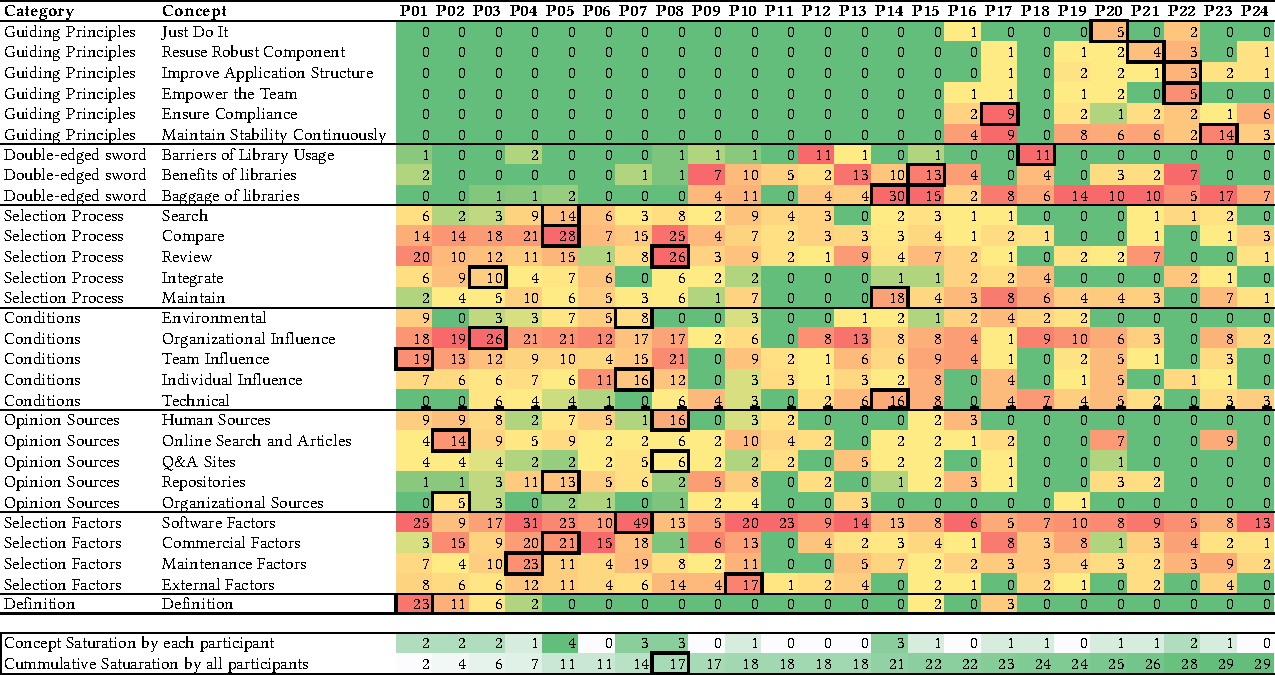
\includegraphics[scale=0.9]{images/saturation.pdf}
    \caption{Heatmap of concept saturation over the interviews. Red refers to the higher discussion of a concept by an interviewee, the number refers to how many times the interviewee has discussed a concept. Green refers to the lower discussion of concepts by an interviewee. Thick black-bordered cells refer to the most discussion reference of a concept among all participants. For example, the review concept under the selection process category was discussed 26 times in P08's interview and hence the corresponding cell is marked by the thick border. The last two rows show the number of concept saturation by each participant and the cumulative number of concepts saturated till that participant. For example, the interview with P08 alone saturated 3 concepts (denoted by the thick boxes in the P08 column) and after the P08 interview, total of 17 concepts were saturated.}
    \label{fig:saturation}
\end{figure*}